\documentclass[12pt]{article}
%	options include 12pt or 11pt or 10pt
%	classes include article, report, book, letter, thesis

% \usepackage[margin=0.75in]{geometry}
\usepackage[margin=0.75in]{geometry}
\setlength{\parindent}{0pt}

\usepackage{hyperref}
\usepackage{amsmath}

%for writing of code in blocks like
%\begin{lstlisting}
%   .......
%\end{lstlisting}
\usepackage{listings}
\usepackage{color}
\usepackage{enumitem}
\usepackage{graphicx}

\definecolor{dkgreen}{rgb}{0,0.6,0}
\definecolor{gray}{rgb}{0.5,0.5,0.5}
\definecolor{mauve}{rgb}{0.58,0,0.82}

\lstset{frame=tb,
  language=C++,
  aboveskip=3mm,
  belowskip=3mm,
  showstringspaces=false,
  columns=flexible,
  basicstyle={\small\ttfamily},
  numbers=none,
  numberstyle=\tiny\color{gray},
  keywordstyle=\color{blue},
  commentstyle=\color{dkgreen},
  stringstyle=\color{mauve},
  breaklines=true,
  breakatwhitespace=true,
  tabsize=3
}
%%%%%%%%%%%%%%%%%%%%%%

\title{Life of a Particle : Quiz 3}
\author{Sam Meehan \& Claire David}
\date{Due Date : 31 January 2019}

\begin{document}
\maketitle

\begin{center}
\begin{LARGE} {\color{red} \textbf{Solutions}} \end{LARGE}\end{center}

% \textbf{Guidelines}:
% \newline
% This quiz will last 15 minutes. Write your answers on paper explaining how you get to the results. 

\section{The unit of charge: the Coulomb}
% The elementary charge carried by the electron is $q_e = 1.6021766208(98) \times 10^{-19}$ C.\\
% Do you know intuitively what is the charge in one Coulomb?
% 
 \begin{figure}[h]
     \centering
     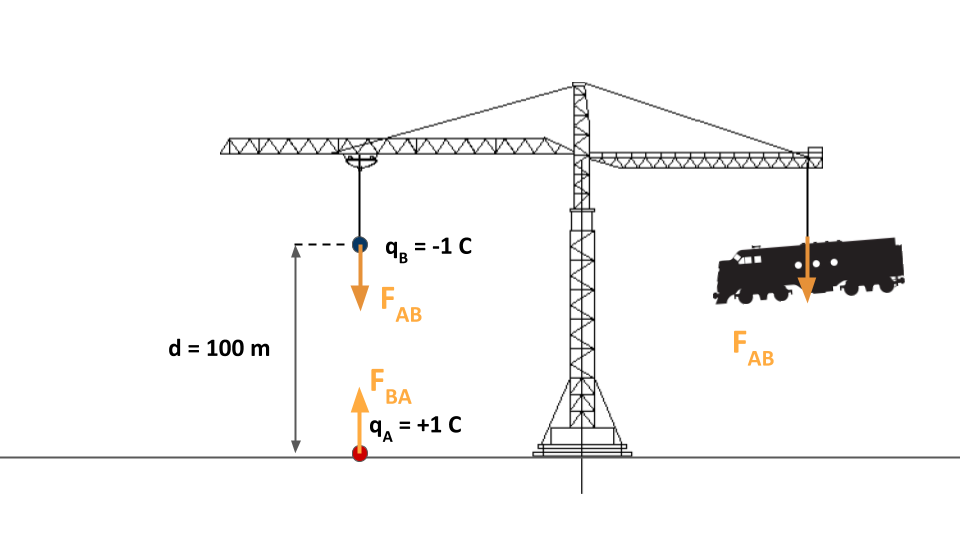
\includegraphics[width=0.8\textwidth]{crane_solution_quiz_part2_1.png}
% %     \caption{}
% %     \label{fig:mesh1}
\end{figure}
% Let's imagine we can fix a positive charge A of one Coulomb in the ground. Let's have a crane where we hang a negative charge B of one Coulomb above the first at a distance $d = 100$ m. The two charges will attract each other, according to the Coulomb force.\\

\textbf{Question A:} What is the mass to be suspended on the other side of the crane to balance this system out? Compare this to a day-to-day life object.\\

{\color{blue}
The two charges will attract each other due to the electrostatic force. Let's compute $\vec{F}_{AB}$, the force exerted by the ground charge on the upper one.
It points downwards and we get the magnitude using Coulomb's law:
\begin{equation}
 \mathbf{F_{AB}} = k_e \frac{q_A \, q_B}{| \, \mathbf{r_{AB}}|^2} \: \mathbf{\hat{r}_{AB}}
\end{equation}
With the values we obtain:
\begin{equation}
 F_{AB} = 8.99 \times 10^9 \, \, \frac{1.00 \times 1.00}{  100 ^2}  = 899 \, \text{kN}
\end{equation}
That's a lot of force. To know the corresponding mass to hang on the other side, we need to have a weight hanging there with the same magnitude as $F_{AB}$. 
With Newton's first law of universal gravitation, we know the weight of an object of mass $m$ on Earth is defined as the force of gravity on the object. It is obtained using the relation:
\begin{equation}
 \vec{F}_\text{grav} = \vec{g} . m
\end{equation}
For the crane to be balanced, we must have $\vec{F}_{AB} = \vec{F}_\text{grav}$. Thus the mass is:
\begin{equation}
 m = \frac{F_\text{grav}}{g} = \frac{F_{AB}}{g} = \frac{899 \times 10^3}{9.81} = 91.6 \times 10^3 \, \text{kg} =  91.6 \, \, \text{tons}
\end{equation}

\textbf{We have to hang a big locomotive to balance two charges of 1 Coulomb separated by 100 metres!}
}
\newline

\textbf{Question B:} A typical lightning strike is about 40 coulombs of charge, consisting of separate "strokes" (that's why lightning usually looks flickery). Each stroke lasts about 30 microseconds. What is the current?\\

{\color{blue}
The current is, by definition, a flow (amount) of charge per unit of time. We have for our strike:
\begin{equation}
 I = \frac{Q}{\Delta t} = \frac{40 }{30 \times 10^{-6} } = 1.33 \times 10^6 \text{A}
\end{equation}

\textbf{Our lightning strike has a current of 1.33 million amperes!}
\newline
To compare, when you charge your smartphone you are using roughly 1 ampere.

}


\section{The electron volt}
% An electron volt (eV) is the energy an electron gains when it is accelerated through a potential difference of one volt. An electron volt is defined as a unit of energy.\\
% 
% A Lindt 70\% cocoa chocolate bar has 194 Calories (one dietary Calorie is 1000 calories, or 4184 Joules).\\
% 
% The LHC operates at 14 TeV (tera eV, 10$^{12}$ eV).\\


\textbf{Question A:} How does the energy of the proton-proton collisions at LHC compare with respect to the energy stored in a cocoa chocolate bar?\\ 

{\color{blue}

Let's convert the energy in the Kingsbite Milk Chocolate Bar in eV:
\begin{equation}
 \frac{ 274 \text{Calories} \times 4184 \text{J/Calorie} }{ 1.6 \cdot 10^{-19} \text{J/eV}} = 7.2 \cdot 10^{24} \text{eV}
\end{equation}
The ratio with the energy in the LHC is:
\begin{equation}
 \frac{7.2 \cdot 10^{24}}{14 \cdot 10^{12}} = 513 \cdot 10^{9}
\end{equation}

\textbf{It would take a 500 billions proton-proton collisions at the LHC top energy to get the same amount of energy as in a Kingsbite Milk Chocolate Bar.}
}\\

\textbf{Question B:} Make the same comparison with energy density.\\

{\color{blue}
The Kingsbite Milk Chocolate Bar has an energy density of about 274 Cal/100 cm$^3$, so 2.74 Cal/cm$^3$.\\
A proton-proton collision at 14 TeV has an energy density around 14 $\cdot 10^{12}$ eV/$10^{-39}$ cm$^3$ $\cdot$ 1.6 $\cdot 10^{-19}$ J/eV $\times$ 4184 Joules. This is 9.4 $\cdot 10^{35}$ Cal/cm$^3$.\\

\begin{center}
\textbf{Proton-proton collisions at the LHC have an energy density about a billion billion billion billion times a Kingsbite Milk Chocolate Bar.}\end{center}
}
    
\end{document}